
\appendix
\section*{Appendix K: Maxwell Fields in Curved Spacetime (Bessel and Hankel Solutions)}

\subsection*{K.1 UBT Motivation and Setting}
In the Unified Biquaternion Theory (UBT), the master field $\Theta(q,\tau)$ lives on a complexified spacetime with $\tau=t+i\psi$.
Electromagnetic (EM) excitations are described by a $U(1)$ sector coupled to $\Theta$, and their propagation in curved geometry is central
for laboratory protocols (Appendix E) and for metric back-reaction studies (Appendix J). Here we develop Maxwell theory on a curved background,
recovering \emph{Bessel} and \emph{Hankel} structures for axisymmetric configurations and summarizing boundary conditions relevant to UBT experiments.

\subsection*{K.2 Maxwell Equations on a Curved Background}
Using metric signature $(-,+,+,+)$, the vacuum Maxwell equations read
\begin{equation}
\nabla_\nu F^{\mu\nu} = \mu_0 J^\mu,\qquad \nabla_{[\alpha} F_{\beta\gamma]}=0,
\end{equation}
with $F_{\mu\nu}=\partial_\mu A_\nu-\partial_\nu A_\mu$, $\nabla$ the Levi--Civita covariant derivative of $g_{\mu\nu}$.
In index-expanded form,
\begin{equation}
\frac{1}{\sqrt{-g}}\partial_\nu\!\left(\sqrt{-g}\,F^{\mu\nu}\right) = \mu_0 J^\mu.
\end{equation}
For stationary, axisymmetric backgrounds (e.g.\ a weakly rotating metric or a cylindrical chart) and harmonic time dependence $e^{-i\omega t}$,
the field equations reduce to scalar Helmholtz-type equations for the longitudinal potentials/components, with a geometry-dependent effective index.

\subsection*{K.3 Cylindrical Separation and Bessel/Hankel Structure}
In cylindrical coordinates $(\rho,\phi,z)$ with axial symmetry and $\partial_z=0$, a representative scalar mode $U(\rho,\phi,t)=R(\rho)\,e^{im\phi}e^{-i\omega t}$ obeys
\begin{equation}
\frac{1}{\rho}\frac{d}{d\rho}\!\left(\rho\,\frac{dR}{d\rho}\right) - \frac{m^2}{\rho^2}R + k_\perp^2 R = 0,\qquad k_\perp^2 = n_{\rm eff}^2(\omega,\text{metric})\,\frac{\omega^2}{c^2},
\end{equation}
with solutions
\begin{equation}
R(\rho) = A\, J_m(k_\perp \rho) + B\, Y_m(k_\perp \rho),\qquad
\text{outgoing waves: } R(\rho)\propto H_m^{(1)}(k_\perp\rho).
\end{equation}
Here $J_m$ and $Y_m$ are Bessel functions of first and second kind; $H_m^{(1)}=J_m+iY_m$ is the outgoing Hankel function.
Curvature and frame-dragging enter $n_{\rm eff}$ and cross-couplings among polarizations (Appendix J).

\subsection*{K.4 Boundary Conditions (PEC Cylinder, TE/TM Selection)}
For a perfect electric conductor (PEC) of radius $a$, the standard boundary conditions yield discrete transverse wavenumbers $k_{\perp,mn}$.
For TM$_{mn}$ (axial $E_z$ nonzero): $J_m(k_{\perp,mn} a)=0$; for TE$_{mn}$ (axial $H_z$ nonzero): $J_m'(k_{\perp,mn} a)=0$.
The lowest zeros are $x_{0,1}\approx 2.4048$ for $J_0$ and $x'_{0,1}=x_{1,1}\approx 3.8317$ for $J'_0$ (i.e.\ the first zero of $J_1$).

\subsection*{K.5 ISM-Band Examples (Radius Estimates)}
For frequency $f$ (wavenumber $k=2\pi f/c$), a cylindrical cavity supporting TM$_{01}$ or TE$_{01}$ has approximate radii $a\approx x_{0,1}/k$ and $a\approx x'_{0,1}/k$, respectively.
Table~\ref{tab:ism_radii} gives indicative values for common ISM bands assuming vacuum ($n_{\rm eff}\!=\!1$). Curved backgrounds shift these via $n_{\rm eff}(\omega)$.
\begin{table}[h!]
\centering
\begin{tabular}{|c|c|c|c|}
\hline
$f$ [GHz] & $k$ [m$^{-1}$] & $a_{\rm TM01}$ [mm] & $a_{\rm TE01}$ [mm] \\
\hline
2.40 & 50.30 & 47.81 & 76.18 \\
5.00 & 104.79 & 22.95 & 36.56 \\
10.00 & 209.58 & 11.47 & 18.28 \\
%
\hline
\end{tabular}
\caption{Indicative cavity radii for TM$_{01}$ ($J_0$ zero) and TE$_{01}$ ($J_0'$ zero) at ISM-like frequencies.}
\label{tab:ism_radii}
\end{table}

\subsection*{K.6 Plots (Embedded Data; No External Figures)}
Figures~\ref{fig:J0J1} and \ref{fig:H0mag} include inline data generated from Bessel and Hankel functions.

\begin{figure}[h!]
\centering
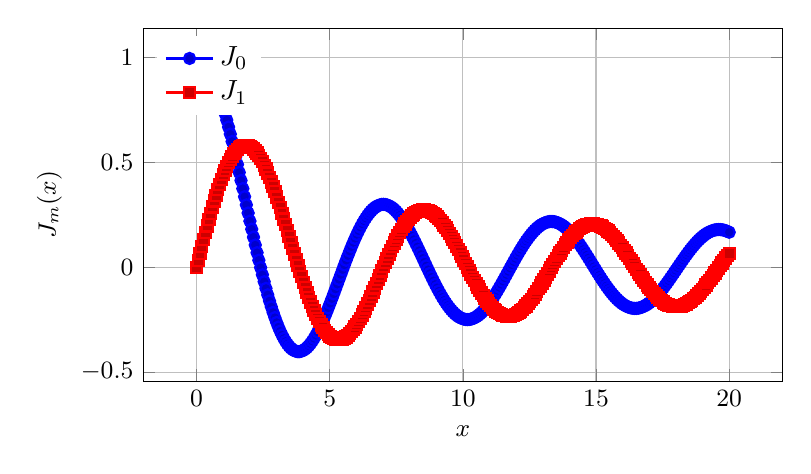
\begin{tikzpicture}
\begin{axis}[width=0.8\textwidth,height=0.5\textwidth,
    xlabel={$x$}, ylabel={$J_m(x)$}, grid=both, legend style={at={(0.02,0.98)},anchor=north west,fill=white,draw=none},
    ticklabel style={font=\small}, label style={font=\small}]
\addplot+[thick] table {
x y
0.000000 1.000000
0.066890 0.998882
0.133779 0.995531
0.200669 0.989958
0.267559 0.982183
0.334448 0.972231
0.401338 0.960136
0.468227 0.945937
0.535117 0.929683
0.602007 0.911429
0.668896 0.891234
0.735786 0.869166
0.802676 0.845299
0.869565 0.819712
0.936455 0.792491
1.003344 0.763724
1.070234 0.733508
1.137124 0.701942
1.204013 0.669131
1.270903 0.635181
1.337793 0.600205
1.404682 0.564316
1.471572 0.527631
1.538462 0.490269
1.605351 0.452351
1.672241 0.413999
1.739130 0.375336
1.806020 0.336485
1.872910 0.297570
1.939799 0.258712
2.006689 0.220035
2.073579 0.181657
2.140468 0.143699
2.207358 0.106275
2.274247 0.069501
2.341137 0.033487
2.408027 -0.001661
2.474916 -0.035838
2.541806 -0.068945
2.608696 -0.100888
2.675585 -0.131577
2.742475 -0.160927
2.809365 -0.188858
2.876254 -0.215297
2.943144 -0.240177
3.010033 -0.263435
3.076923 -0.285017
3.143813 -0.304873
3.210702 -0.322962
3.277592 -0.339249
3.344482 -0.353704
3.411371 -0.366307
3.478261 -0.377042
3.545151 -0.385903
3.612040 -0.392888
3.678930 -0.398004
3.745819 -0.401264
3.812709 -0.402687
3.879599 -0.402299
3.946488 -0.400135
4.013378 -0.396232
4.080268 -0.390637
4.147157 -0.383399
4.214047 -0.374576
4.280936 -0.364229
4.347826 -0.352427
4.414716 -0.339241
4.481605 -0.324747
4.548495 -0.309026
4.615385 -0.292163
4.682274 -0.274244
4.749164 -0.255363
4.816054 -0.235611
4.882943 -0.215085
4.949833 -0.193882
5.016722 -0.172103
5.083612 -0.149848
5.150502 -0.127218
5.217391 -0.104315
5.284281 -0.081240
5.351171 -0.058094
5.418060 -0.034977
5.484950 -0.011989
5.551839 0.010774
5.618729 0.033217
5.685619 0.055246
5.752508 0.076772
5.819398 0.097708
5.886288 0.117970
5.953177 0.137479
6.020067 0.156158
6.086957 0.173935
6.153846 0.190745
6.220736 0.206525
6.287625 0.221217
6.354515 0.234770
6.421405 0.247136
6.488294 0.258274
6.555184 0.268149
6.622074 0.276731
6.688963 0.283994
6.755853 0.289922
6.822742 0.294501
6.889632 0.297724
6.956522 0.299591
7.023411 0.300107
7.090301 0.299281
7.157191 0.297132
7.224080 0.293679
7.290970 0.288951
7.357860 0.282980
7.424749 0.275803
7.491639 0.267462
7.558528 0.258004
7.625418 0.247481
7.692308 0.235948
7.759197 0.223463
7.826087 0.210091
7.892977 0.195897
7.959866 0.180950
8.026756 0.165323
8.093645 0.149089
8.160535 0.132324
8.227425 0.115107
8.294314 0.097516
8.361204 0.079632
8.428094 0.061536
8.494983 0.043309
8.561873 0.025032
8.628763 0.006786
8.695652 -0.011350
8.762542 -0.029296
8.829431 -0.046975
8.896321 -0.064311
8.963211 -0.081231
9.030100 -0.097663
9.096990 -0.113539
9.163880 -0.128792
9.230769 -0.143361
9.297659 -0.157186
9.364548 -0.170210
9.431438 -0.182384
9.498328 -0.193659
9.565217 -0.203991
9.632107 -0.213343
9.698997 -0.221678
9.765886 -0.228969
9.832776 -0.235189
9.899666 -0.240318
9.966555 -0.244342
10.033445 -0.247250
10.100334 -0.249036
10.167224 -0.249700
10.234114 -0.249247
10.301003 -0.247685
10.367893 -0.245030
10.434783 -0.241299
10.501672 -0.236516
10.568562 -0.230709
10.635452 -0.223910
10.702341 -0.216156
10.769231 -0.207486
10.836120 -0.197944
10.903010 -0.187579
10.969900 -0.176440
11.036789 -0.164583
11.103679 -0.152063
11.170569 -0.138941
11.237458 -0.125277
11.304348 -0.111136
11.371237 -0.096583
11.438127 -0.081684
11.505017 -0.066508
11.571906 -0.051123
11.638796 -0.035599
11.705686 -0.020005
11.772575 -0.004411
11.839465 0.011115
11.906355 0.026504
11.973244 0.041688
12.040134 0.056601
12.107023 0.071180
12.173913 0.085361
12.240803 0.099083
12.307692 0.112288
12.374582 0.124922
12.441472 0.136929
12.508361 0.148262
12.575251 0.158873
12.642140 0.168719
12.709030 0.177760
12.775920 0.185961
12.842809 0.193290
12.909699 0.199718
12.976589 0.205222
13.043478 0.209782
13.110368 0.213383
13.177258 0.216014
13.244147 0.217668
13.311037 0.218342
13.377926 0.218039
13.444816 0.216764
13.511706 0.214529
13.578595 0.211348
13.645485 0.207239
13.712375 0.202226
13.779264 0.196335
13.846154 0.189597
13.913043 0.182045
13.979933 0.173717
14.046823 0.164654
14.113712 0.154899
14.180602 0.144499
14.247492 0.133503
14.314381 0.121963
14.381271 0.109933
14.448161 0.097468
14.515050 0.084625
14.581940 0.071464
14.648829 0.058045
14.715719 0.044427
14.782609 0.030673
14.849498 0.016844
14.916388 0.003002
14.983278 -0.010791
15.050167 -0.024475
15.117057 -0.037988
15.183946 -0.051273
15.250836 -0.064270
15.317726 -0.076924
15.384615 -0.089179
15.451505 -0.100984
15.518395 -0.112286
15.585284 -0.123039
15.652174 -0.133196
15.719064 -0.142716
15.785953 -0.151558
15.852843 -0.159687
15.919732 -0.167069
15.986622 -0.173674
16.053512 -0.179476
16.120401 -0.184453
16.187291 -0.188586
16.254181 -0.191861
16.321070 -0.194266
16.387960 -0.195793
16.454849 -0.196441
16.521739 -0.196209
16.588629 -0.195102
16.655518 -0.193129
16.722408 -0.190302
16.789298 -0.186637
16.856187 -0.182153
16.923077 -0.176874
16.989967 -0.170826
17.056856 -0.164039
17.123746 -0.156547
17.190635 -0.148385
17.257525 -0.139592
17.324415 -0.130211
17.391304 -0.120284
17.458194 -0.109858
17.525084 -0.098982
17.591973 -0.087706
17.658863 -0.076080
17.725753 -0.064159
17.792642 -0.051997
17.859532 -0.039648
17.926421 -0.027168
17.993311 -0.014613
18.060201 -0.002040
18.127090 0.010496
18.193980 0.022939
18.260870 0.035234
18.327759 0.047326
18.394649 0.059164
18.461538 0.070694
18.528428 0.081866
18.595318 0.092634
18.662207 0.102948
18.729097 0.112767
18.795987 0.122047
18.862876 0.130749
18.929766 0.138836
18.996656 0.146275
19.063545 0.153035
19.130435 0.159088
19.197324 0.164409
19.264214 0.168978
19.331104 0.172777
19.397993 0.175791
19.464883 0.178010
19.531773 0.179426
19.598662 0.180037
19.665552 0.179841
19.732441 0.178843
19.799331 0.177051
19.866221 0.174473
19.933110 0.171125
20.000000 0.167025
};
\addlegendentry{$J_0$}
\addplot+[thick] table {
x y
0.000000 0.000000
0.066890 0.033426
0.133779 0.066740
0.200669 0.099830
0.267559 0.132586
0.334448 0.164897
0.401338 0.196656
0.468227 0.227756
0.535117 0.258095
0.602007 0.287572
0.668896 0.316089
0.735786 0.343552
0.802676 0.369872
0.869565 0.394962
0.936455 0.418743
1.003344 0.441136
1.070234 0.462072
1.137124 0.481484
1.204013 0.499313
1.270903 0.515504
1.337793 0.530009
1.404682 0.542785
1.471572 0.553798
1.538462 0.563017
1.605351 0.570421
1.672241 0.575993
1.739130 0.579724
1.806020 0.581611
1.872910 0.581659
1.939799 0.579878
2.006689 0.576285
2.073579 0.570904
2.140468 0.563765
2.207358 0.554905
2.274247 0.544367
2.341137 0.532199
2.408027 0.518455
2.474916 0.503194
2.541806 0.486483
2.608696 0.468391
2.675585 0.448992
2.742475 0.428366
2.809365 0.406596
2.876254 0.383768
2.943144 0.359974
3.010033 0.335307
3.076923 0.309862
3.143813 0.283738
3.210702 0.257036
3.277592 0.229857
3.344482 0.202304
3.411371 0.174481
3.478261 0.146492
3.545151 0.118441
3.612040 0.090431
3.678930 0.062566
3.745819 0.034945
3.812709 0.007670
3.879599 -0.019163
3.946488 -0.045457
4.013378 -0.071121
4.080268 -0.096065
4.147157 -0.120203
4.214047 -0.143452
4.280936 -0.165734
4.347826 -0.186975
4.414716 -0.207106
4.481605 -0.226062
4.548495 -0.243783
4.615385 -0.260216
4.682274 -0.275310
4.749164 -0.289024
4.816054 -0.301320
4.882943 -0.312165
4.949833 -0.321533
5.016722 -0.329406
5.083612 -0.335769
5.150502 -0.340615
5.217391 -0.343942
5.284281 -0.345754
5.351171 -0.346061
5.418060 -0.344880
5.484950 -0.342233
5.551839 -0.338147
5.618729 -0.332656
5.685619 -0.325797
5.752508 -0.317614
5.819398 -0.308157
5.886288 -0.297477
5.953177 -0.285634
6.020067 -0.272688
6.086957 -0.258706
6.153846 -0.243757
6.220736 -0.227914
6.287625 -0.211253
6.354515 -0.193852
6.421405 -0.175792
6.488294 -0.157156
6.555184 -0.138028
6.622074 -0.118495
6.688963 -0.098642
6.755853 -0.078558
6.822742 -0.058330
6.889632 -0.038046
6.956522 -0.017791
7.023411 0.002347
7.090301 0.022284
7.157191 0.041937
7.224080 0.061223
7.290970 0.080065
7.357860 0.098385
7.424749 0.116109
7.491639 0.133167
7.558528 0.149490
7.625418 0.165016
7.692308 0.179683
7.759197 0.193438
7.826087 0.206227
7.892977 0.218003
7.959866 0.228725
8.026756 0.238355
8.093645 0.246859
8.160535 0.254211
8.227425 0.260388
8.294314 0.265371
8.361204 0.269150
8.428094 0.271716
8.494983 0.273069
8.561873 0.273212
8.628763 0.272153
8.695652 0.269906
8.762542 0.266489
8.829431 0.261927
8.896321 0.256247
8.963211 0.249482
9.030100 0.241669
9.096990 0.232851
9.163880 0.223071
9.230769 0.212381
9.297659 0.200833
9.364548 0.188483
9.431438 0.175390
9.498328 0.161617
9.565217 0.147228
9.632107 0.132291
9.698997 0.116873
9.765886 0.101046
9.832776 0.084882
9.899666 0.068453
9.966555 0.051832
10.033445 0.035094
10.100334 0.018312
10.167224 0.001560
10.234114 -0.015089
10.301003 -0.031563
10.367893 -0.047791
10.434783 -0.063704
10.501672 -0.079233
10.568562 -0.094314
10.635452 -0.108883
10.702341 -0.122879
10.769231 -0.136245
10.836120 -0.148926
10.903010 -0.160871
10.969900 -0.172031
11.036789 -0.182363
11.103679 -0.191826
11.170569 -0.200383
11.237458 -0.208003
11.304348 -0.214658
11.371237 -0.220323
11.438127 -0.224981
11.505017 -0.228615
11.571906 -0.231217
11.638796 -0.232781
11.705686 -0.233304
11.772575 -0.232792
11.839465 -0.231253
11.906355 -0.228697
11.973244 -0.225144
12.040134 -0.220613
12.107023 -0.215129
12.173913 -0.208723
12.240803 -0.201428
12.307692 -0.193280
12.374582 -0.184319
12.441472 -0.174590
12.508361 -0.164140
12.575251 -0.153017
12.642140 -0.141276
12.709030 -0.128970
12.775920 -0.116157
12.842809 -0.102896
12.909699 -0.089248
12.976589 -0.075274
13.043478 -0.061038
13.110368 -0.046605
13.177258 -0.032038
13.244147 -0.017403
13.311037 -0.002765
13.377926 0.011813
13.444816 0.026265
13.511706 0.040529
13.578595 0.054543
13.645485 0.068246
13.712375 0.081579
13.779264 0.094485
13.846154 0.106909
13.913043 0.118799
13.979933 0.130105
14.046823 0.140779
14.113712 0.150777
14.180602 0.160059
14.247492 0.168586
14.314381 0.176325
14.381271 0.183245
14.448161 0.189319
14.515050 0.194524
14.581940 0.198841
14.648829 0.202256
14.715719 0.204756
14.782609 0.206336
14.849498 0.206992
14.916388 0.206726
14.983278 0.205542
15.050167 0.203451
15.117057 0.200465
15.183946 0.196601
15.250836 0.191881
15.317726 0.186329
15.384615 0.179973
15.451505 0.172844
15.518395 0.164979
15.585284 0.156414
15.652174 0.147190
15.719064 0.137352
15.785953 0.126945
15.852843 0.116017
15.919732 0.104620
15.986622 0.092805
16.053512 0.080628
16.120401 0.068142
16.187291 0.055405
16.254181 0.042474
16.321070 0.029408
16.387960 0.016264
16.454849 0.003102
16.521739 -0.010021
16.588629 -0.023047
16.655518 -0.035917
16.722408 -0.048576
16.789298 -0.060969
16.856187 -0.073041
16.923077 -0.084740
16.989967 -0.096017
17.056856 -0.106821
17.123746 -0.117109
17.190635 -0.126835
17.257525 -0.135959
17.324415 -0.144444
17.391304 -0.152252
17.458194 -0.159354
17.525084 -0.165719
17.591973 -0.171323
17.658863 -0.176143
17.725753 -0.180161
17.792642 -0.183362
17.859532 -0.185735
17.926421 -0.187273
17.993311 -0.187971
18.060201 -0.187831
18.127090 -0.186855
18.193980 -0.185051
18.260870 -0.182429
18.327759 -0.179006
18.394649 -0.174798
18.461538 -0.169828
18.528428 -0.164119
18.595318 -0.157700
18.662207 -0.150603
18.729097 -0.142860
18.795987 -0.134509
18.862876 -0.125589
18.929766 -0.116141
18.996656 -0.106210
19.063545 -0.095840
19.130435 -0.085081
19.197324 -0.073979
19.264214 -0.062587
19.331104 -0.050956
19.397993 -0.039139
19.464883 -0.027187
19.531773 -0.015156
19.598662 -0.003098
19.665552 0.008933
19.732441 0.020883
19.799331 0.032699
19.866221 0.044330
19.933110 0.055725
20.000000 0.066833
};
\addlegendentry{$J_1$}
\end{axis}
\end{tikzpicture}
\caption{Bessel functions $J_0$ and $J_1$ relevant for TM/TE mode selection in cylindrical symmetry.}
\label{fig:J0J1}
\end{figure}

\begin{figure}[h!]
\centering
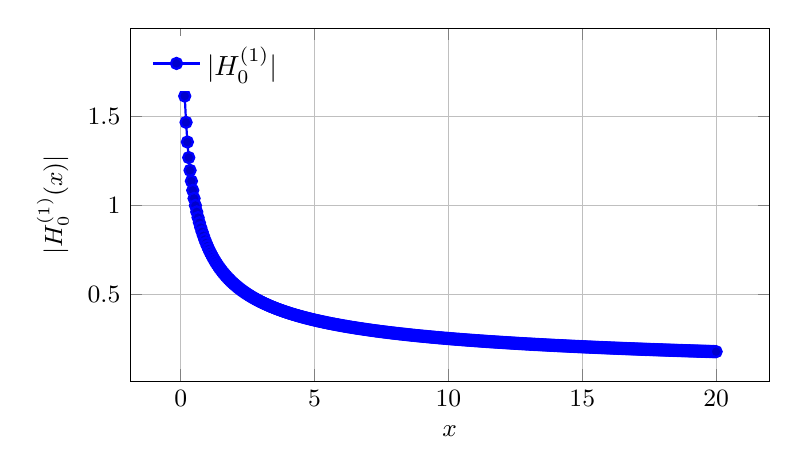
\begin{tikzpicture}
\begin{axis}[width=0.8\textwidth,height=0.5\textwidth,
    xlabel={$x$}, ylabel={$|H_0^{(1)}(x)|$}, grid=both, legend style={at={(0.02,0.98)},anchor=north west,fill=white,draw=none},
    ticklabel style={font=\small}, label style={font=\small}]
\addplot+[thick] table {
x y
0.100000 1.829999
0.149875 1.614026
0.199749 1.466557
0.249624 1.356072
0.299499 1.268640
0.349373 1.196891
0.399248 1.136459
0.449123 1.084551
0.498997 1.039275
0.548872 0.999292
0.598747 0.963620
0.648622 0.931522
0.698496 0.902428
0.748371 0.875889
0.798246 0.851547
0.848120 0.829113
0.897995 0.808346
0.947870 0.789050
0.997744 0.771056
1.047619 0.754225
1.097494 0.738435
1.147368 0.723584
1.197243 0.709582
1.247118 0.696351
1.296992 0.683822
1.346867 0.671937
1.396742 0.660641
1.446617 0.649888
1.496491 0.639636
1.546366 0.629847
1.596241 0.620487
1.646115 0.611527
1.695990 0.602938
1.745865 0.594696
1.795739 0.586778
1.845614 0.579164
1.895489 0.571834
1.945363 0.564772
1.995238 0.557962
2.045113 0.551389
2.094987 0.545040
2.144862 0.538902
2.194737 0.532965
2.244612 0.527217
2.294486 0.521649
2.344361 0.516251
2.394236 0.511016
2.444110 0.505935
2.493985 0.501000
2.543860 0.496206
2.593734 0.491545
2.643609 0.487012
2.693484 0.482600
2.743358 0.478305
2.793233 0.474121
2.843108 0.470045
2.892982 0.466070
2.942857 0.462194
2.992732 0.458411
3.042607 0.454720
3.092481 0.451115
3.142356 0.447594
3.192231 0.444153
3.242105 0.440790
3.291980 0.437501
3.341855 0.434284
3.391729 0.431136
3.441604 0.428056
3.491479 0.425040
3.541353 0.422086
3.591228 0.419193
3.641103 0.416357
3.690977 0.413579
3.740852 0.410854
3.790727 0.408183
3.840602 0.405562
3.890476 0.402991
3.940351 0.400468
3.990226 0.397991
4.040100 0.395559
4.089975 0.393172
4.139850 0.390826
4.189724 0.388522
4.239599 0.386258
4.289474 0.384032
4.339348 0.381845
4.389223 0.379694
4.439098 0.377579
4.488972 0.375499
4.538847 0.373452
4.588722 0.371439
4.638596 0.369457
4.688471 0.367507
4.738346 0.365587
4.788221 0.363697
4.838095 0.361835
4.887970 0.360002
4.937845 0.358196
4.987719 0.356417
5.037594 0.354664
5.087469 0.352936
5.137343 0.351234
5.187218 0.349555
5.237093 0.347901
5.286967 0.346269
5.336842 0.344661
5.386717 0.343074
5.436591 0.341509
5.486466 0.339965
5.536341 0.338442
5.586216 0.336939
5.636090 0.335455
5.685965 0.333991
5.735840 0.332546
5.785714 0.331120
5.835589 0.329711
5.885464 0.328321
5.935338 0.326948
5.985213 0.325591
6.035088 0.324252
6.084962 0.322929
6.134837 0.321621
6.184712 0.320330
6.234586 0.319054
6.284461 0.317793
6.334336 0.316546
6.384211 0.315315
6.434085 0.314097
6.483960 0.312894
6.533835 0.311704
6.583709 0.310527
6.633584 0.309364
6.683459 0.308214
6.733333 0.307076
6.783208 0.305951
6.833083 0.304838
6.882957 0.303737
6.932832 0.302648
6.982707 0.301570
7.032581 0.300504
7.082456 0.299449
7.132331 0.298405
7.182206 0.297372
7.232080 0.296350
7.281955 0.295337
7.331830 0.294336
7.381704 0.293344
7.431579 0.292362
7.481454 0.291390
7.531328 0.290428
7.581203 0.289475
7.631078 0.288531
7.680952 0.287597
7.730827 0.286671
7.780702 0.285755
7.830576 0.284847
7.880451 0.283947
7.930326 0.283057
7.980201 0.282174
8.030075 0.281300
8.079950 0.280433
8.129825 0.279575
8.179699 0.278724
8.229574 0.277881
8.279449 0.277046
8.329323 0.276218
8.379198 0.275398
8.429073 0.274585
8.478947 0.273779
8.528822 0.272980
8.578697 0.272188
8.628571 0.271402
8.678446 0.270624
8.728321 0.269852
8.778195 0.269087
8.828070 0.268328
8.877945 0.267575
8.927820 0.266829
8.977694 0.266089
9.027569 0.265355
9.077444 0.264628
9.127318 0.263906
9.177193 0.263190
9.227068 0.262479
9.276942 0.261775
9.326817 0.261076
9.376692 0.260383
9.426566 0.259695
9.476441 0.259012
9.526316 0.258335
9.576190 0.257663
9.626065 0.256997
9.675940 0.256335
9.725815 0.255679
9.775689 0.255027
9.825564 0.254381
9.875439 0.253739
9.925313 0.253103
9.975188 0.252471
10.025063 0.251843
10.074937 0.251221
10.124812 0.250603
10.174687 0.249989
10.224561 0.249380
10.274436 0.248776
10.324311 0.248175
10.374185 0.247579
10.424060 0.246988
10.473935 0.246400
10.523810 0.245817
10.573684 0.245238
10.623559 0.244663
10.673434 0.244092
10.723308 0.243525
10.773183 0.242961
10.823058 0.242402
10.872932 0.241847
10.922807 0.241295
10.972682 0.240747
11.022556 0.240203
11.072431 0.239662
11.122306 0.239126
11.172180 0.238592
11.222055 0.238063
11.271930 0.237536
11.321805 0.237013
11.371679 0.236494
11.421554 0.235978
11.471429 0.235466
11.521303 0.234956
11.571178 0.234450
11.621053 0.233948
11.670927 0.233448
11.720802 0.232952
11.770677 0.232459
11.820551 0.231969
11.870426 0.231482
11.920301 0.230998
11.970175 0.230517
12.020050 0.230039
12.069925 0.229564
12.119799 0.229092
12.169674 0.228623
12.219549 0.228156
12.269424 0.227693
12.319298 0.227232
12.369173 0.226774
12.419048 0.226319
12.468922 0.225867
12.518797 0.225417
12.568672 0.224970
12.618546 0.224526
12.668421 0.224084
12.718296 0.223645
12.768170 0.223209
12.818045 0.222775
12.867920 0.222343
12.917794 0.221914
12.967669 0.221487
13.017544 0.221063
13.067419 0.220642
13.117293 0.220222
13.167168 0.219806
13.217043 0.219391
13.266917 0.218979
13.316792 0.218569
13.366667 0.218161
13.416541 0.217756
13.466416 0.217353
13.516291 0.216952
13.566165 0.216554
13.616040 0.216157
13.665915 0.215763
13.715789 0.215371
13.765664 0.214981
13.815539 0.214593
13.865414 0.214207
13.915288 0.213823
13.965163 0.213442
14.015038 0.213062
14.064912 0.212684
14.114787 0.212309
14.164662 0.211935
14.214536 0.211563
14.264411 0.211194
14.314286 0.210826
14.364160 0.210460
14.414035 0.210096
14.463910 0.209734
14.513784 0.209374
14.563659 0.209015
14.613534 0.208659
14.663409 0.208304
14.713283 0.207951
14.763158 0.207600
14.813033 0.207250
14.862907 0.206903
14.912782 0.206557
14.962657 0.206213
15.012531 0.205870
15.062406 0.205529
15.112281 0.205190
15.162155 0.204853
15.212030 0.204517
15.261905 0.204183
15.311779 0.203851
15.361654 0.203520
15.411529 0.203191
15.461404 0.202863
15.511278 0.202537
15.561153 0.202212
15.611028 0.201889
15.660902 0.201568
15.710777 0.201248
15.760652 0.200930
15.810526 0.200613
15.860401 0.200298
15.910276 0.199984
15.960150 0.199671
16.010025 0.199360
16.059900 0.199051
16.109774 0.198743
16.159649 0.198436
16.209524 0.198131
16.259398 0.197827
16.309273 0.197525
16.359148 0.197224
16.409023 0.196924
16.458897 0.196626
16.508772 0.196329
16.558647 0.196033
16.608521 0.195739
16.658396 0.195446
16.708271 0.195154
16.758145 0.194864
16.808020 0.194575
16.857895 0.194287
16.907769 0.194000
16.957644 0.193715
17.007519 0.193431
17.057393 0.193148
17.107268 0.192867
17.157143 0.192587
17.207018 0.192307
17.256892 0.192030
17.306767 0.191753
17.356642 0.191477
17.406516 0.191203
17.456391 0.190930
17.506266 0.190658
17.556140 0.190387
17.606015 0.190118
17.655890 0.189849
17.705764 0.189582
17.755639 0.189316
17.805514 0.189050
17.855388 0.188786
17.905263 0.188523
17.955138 0.188262
18.005013 0.188001
18.054887 0.187741
18.104762 0.187483
18.154637 0.187225
18.204511 0.186969
18.254386 0.186713
18.304261 0.186459
18.354135 0.186206
18.404010 0.185953
18.453885 0.185702
18.503759 0.185452
18.553634 0.185203
18.603509 0.184954
18.653383 0.184707
18.703258 0.184461
18.753133 0.184216
18.803008 0.183971
18.852882 0.183728
18.902757 0.183486
18.952632 0.183244
19.002506 0.183004
19.052381 0.182764
19.102256 0.182526
19.152130 0.182288
19.202005 0.182051
19.251880 0.181815
19.301754 0.181580
19.351629 0.181346
19.401504 0.181113
19.451378 0.180881
19.501253 0.180650
19.551128 0.180419
19.601003 0.180190
19.650877 0.179961
19.700752 0.179733
19.750627 0.179507
19.800501 0.179280
19.850376 0.179055
19.900251 0.178831
19.950125 0.178607
20.000000 0.178385
};
\addlegendentry{$|H_0^{(1)}|$}
\end{axis}
\end{tikzpicture}
\caption{Magnitude of the outgoing Hankel function $H_0^{(1)}=J_0+iY_0$.}
\label{fig:H0mag}
\end{figure}

\subsection*{K.7 Curved-Space Corrections and UBT Links}
Weak curvature and frame-dragging modify the separation constant via an effective index $n_{\rm eff}(\omega,\text{metric})$ and couple polarizations in the transport equations (eikonal limit).
Within UBT, slow $\psi$-sector deformations shift dispersion and boundary spectra ($k_{\perp,mn}\to k_{\perp,mn}+\delta k_{\perp}(\psi)$), yielding measurable changes in cavity frequencies and
scattering phase (cross-reference: Appendix I, J, E). These provide direct targets for metrology and for bounding the $\psi$-sector couplings.

\subsection*{K.8 Summary}
Maxwell fields on curved backgrounds separate to Bessel/Hankel radial profiles under axial symmetry.
PEC boundaries quantize $k_\perp$ via zeros of $J_m$ or $J_m'$; curved-space and UBT $\psi$-sector effects enter as shifts of the effective index and mode spectrum.
The ISM-band radius estimates connect theory to buildable experiments, while embedded plots serve as quick references for $J_0, J_1$, and $|H_0^{(1)}|$.
